\begin{figure}[h]
\begin{center}
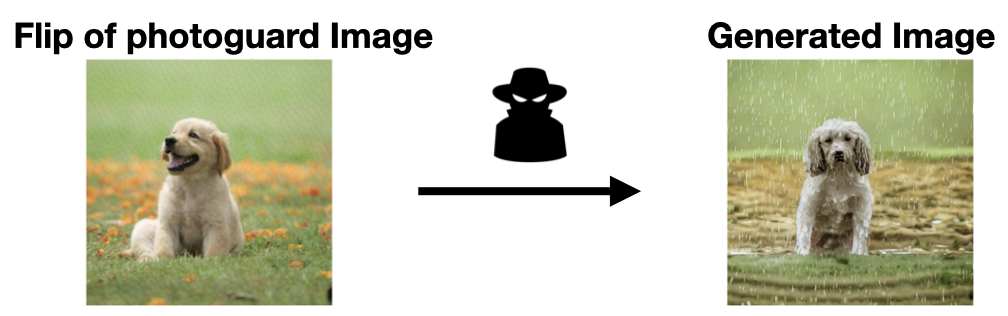
\includegraphics[width=0.58\textwidth]{images/flip-and-blur-figures.001.png}
\end{center}
\caption{\textbf{Flip of photoguard image}. Left: We perform a horizontal flip on a photoguard image. Right: Starting from the flipped image, the adversary uses a diffusion model to make edits according to the same prompt setup as Figure~\ref{fig:img2img-overview}. The generated image does not retain the original subject.}
\label{figure-flip}
\end{figure}